\begin{frame}[t]
    \begin{theorem}[D.König, 1931]
        В двудольном графе $G = \left( L, R, E \right): \alpha'(G) = \beta(G)$.
    \end{theorem}

    \begin{proof}[Доказательство]
        \renewcommand{\qedsymbol}{}
        Будем доказывать теорему при помощи теоремы Холла.
        \begin{itemize}
            \item Рассмотрим наименьшее вершинное покрытие (обозначим $B, \beta(G) = |B|$). Перестроим двудольный граф следующим образом: $G' = \left(B, V(G) \backslash B, E'\right)$ (в левую долу поместим выбранные в $B$ вершины, остальные поместим в правую).
            \item В правой доле рёбер нет: иначе $B$ не является вершинным покрытием. Удалим все рёбра между вершинами левой доли -- если мы докажем, что $\alpha'(G') \geq \beta(G)$, то и $\alpha'(G) \geq \alpha'(G') \geq \beta(G)$ (новых рёбер в граф не добавлялось)
        \end{itemize}
          
    \end{proof}
\end{frame}

\begin{frame}[t]
    \begin{figure}[htpb]
        \centering
        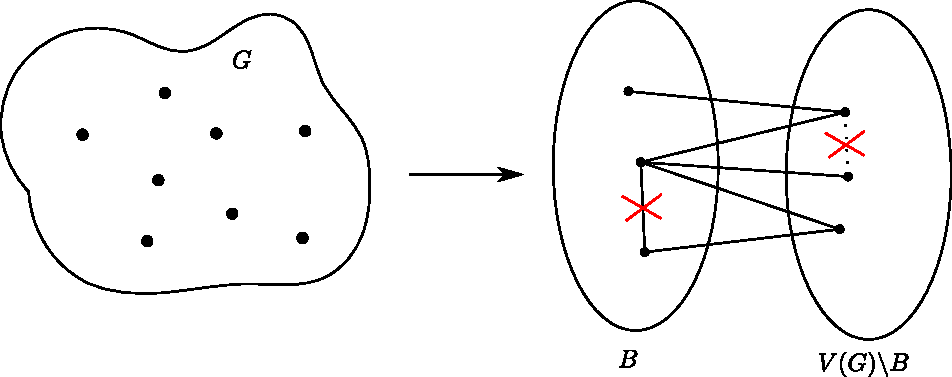
\includegraphics[width=\textwidth]{images/transform}
        \footnotesize Преобразование графа
        \label{fig:transform}
    \end{figure}
    
    \begin{itemize}
        \item Для того, чтобы доказать, что $\alpha'(G) = \beta(G)$, достаточно доказать, что $\alpha'(G) \geq \beta(G)$ и $\alpha'(G) \leq \beta(G)$.
    \end{itemize}
    
\end{frame}

\begin{frame}[t]
    \small
    \frametitle{$\alpha'(G) \geq \beta(G)$}
    \begin{itemize}
        \item Проверим наличие паросочетания размера $|B| = \beta(G)$. Достаточно проверить условие Холла для $B$.
        \item Если это не так, то $\exists S \subset B: |N_{G'}(S)| < |S|$ и, заменив \textcolor{blue}{$S$} на \textcolor{red}{$N_G(S)$}, мы получим, что множество рёбер, которое покрывается, остаётся прежним ($ \Rightarrow $ условие для покрытия сохраняется), а размер покрытия станет меньше, противоречие с минимальностью $B$. 
    \end{itemize}
    \vspace{-5mm}
    \begin{figure}[h]
        \centering
        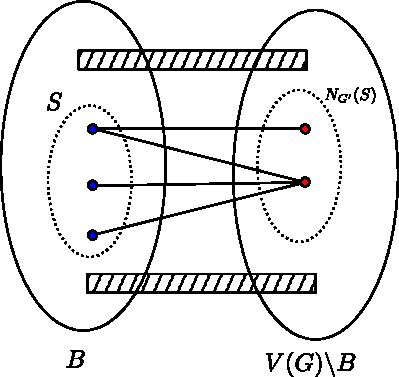
\includegraphics[width=0.45\textwidth]{images/hall}
        \label{fig:hall}
    \end{figure}
    
\end{frame}

\begin{frame}[t]
    \small
    \frametitle{$\alpha'(G) \leq \beta(G)$}

    \begin{itemize}
        \item Для каждого ребра из максимального паросочетания $M$ при покрытии среди двух вершин ребра $e \in M$ нужно выбрать хотя бы одну.
        \item В противном случае ребро $e$ не будет покрыто.
        \item Таким образом, $\beta(G) \geq \alpha' (G)$. 
    \end{itemize}
    \hfill \qedsymbol
\end{frame}

